%% building_to_metabolism.tex
%% Author: Leighton Pritchard
%% Copyright: James Hutton Institute
%% A brief introduction to orthologues, and evaluation of their prediction

% SUBSECTION: Reconstructing metabolism
\subsection{Reconstructing metabolism}

% Which methods work best
\begin{frame}
  \frametitle{Reconstructing metabolism\footnote{\tiny{Thiele and Palsson (2010) \textit{Nat. Protoc.} \textbf{5}:93-121 \href{http://dx.doi.org/10.1038/nprot.2009.203}{doi:10.1038/nprot.2009.203}}}}
  Once metabolic functional annotation has been assigned to features, we can do comparative analysis of metabolism.
  \begin{center}
      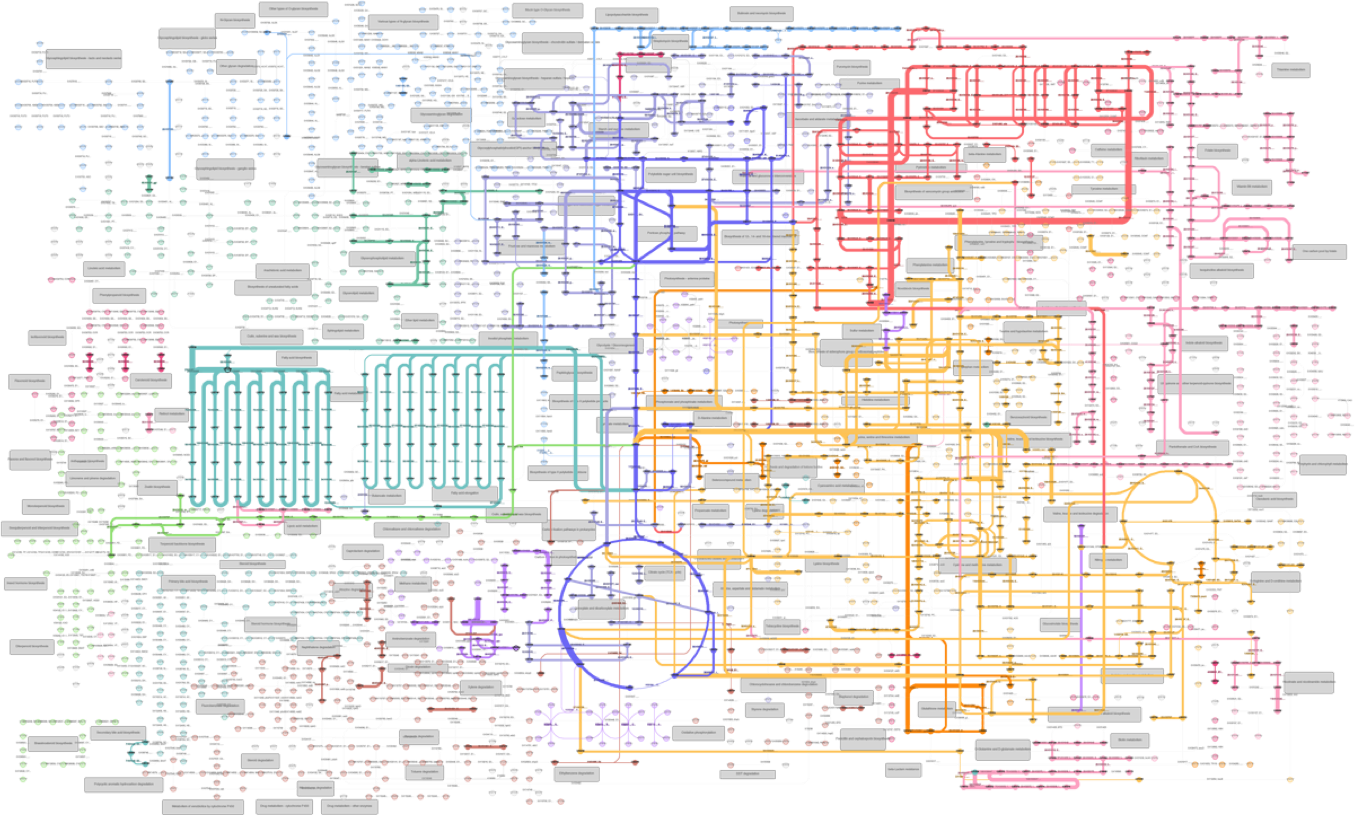
\includegraphics[width=1\textwidth]{images/dickeya_metabolism} 
  \end{center}
\end{frame}

% Which methods work best
\begin{frame}
  \frametitle{Dynamic models of metabolism\footnote{\tiny{Orth \textit{et al.} (2010) \textit{Nat. Biotech.} \textbf{28}:245-248 \href{http://dx.doi.org/10.1038/nbt.1614}{doi:10.1038/nbt.1614}}}}
  By using constraint-based models (e.g. Flux Balance Analysis), we can make these into dynamic representations of bacterial metabolism.
  \begin{itemize}
    \item Upper, lower bounds to reaction rates
    \item Define objective phenotype
    \item Calculate conditions resulting in flux
    \item \textit{in silico} knockouts
  \end{itemize}
  \begin{center}
      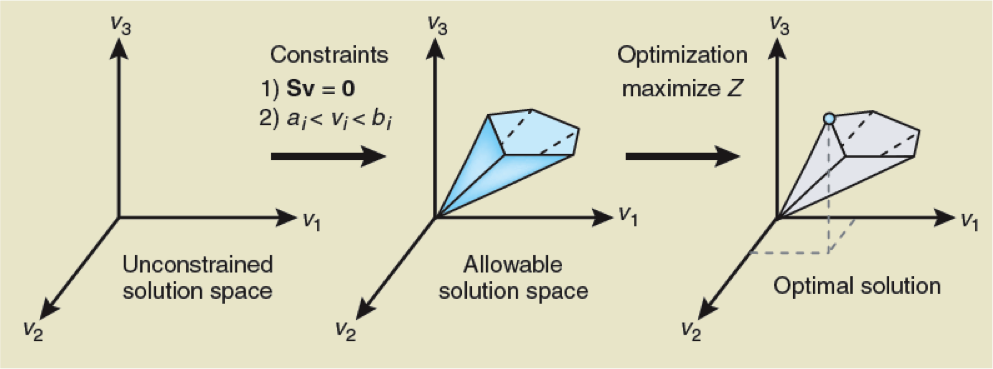
\includegraphics[width=1\textwidth]{images/fba} 
  \end{center}
\end{frame}

% Which methods work best
\begin{frame}
  \frametitle{\textit{E. coli} metabolism\footnote{\tiny{Monk \textit{et al.} (2013) \textit{Proc. Natl. Acad. Sci. USA} \textbf{110}:20338-20343 \href{http://dx.doi.org/10.1073/pnas.1307797110}{doi:10.1073/pnas.1307797110}}}}
  \textit{E. coli} has a very long history of metabolic reconstruction\footnote{\tiny{Reed and Palsson (2000) \textit{J. Bact.} \textbf{185}:2692-2699 \href{http://dx.doi.org/10.1128/JB.185.9.2692-2699.2003}{doi:10.1128/JB.185.9.2692-2699.2003}}}\\
  Recent modelling work predicts which nutrients support growth
  \begin{center}
      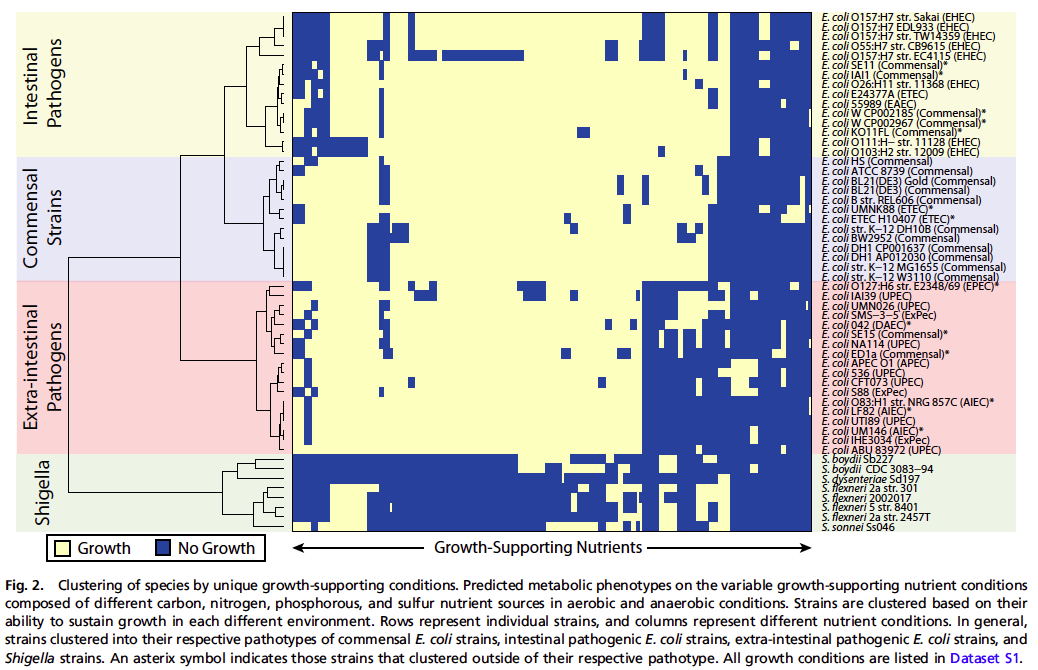
\includegraphics[width=0.85\textwidth]{images/e_coli_growth} 
  \end{center}
\end{frame}

% Which methods work best
\begin{frame}
  \frametitle{\textit{E. coli} metabolism\footnote{\tiny{Baumler \textit{et al.} (2011) \textit{BMC Syst. Biol.} \textbf{5}:182 \href{http://dx.doi.org/10.1186/1752-0509-5-182}{doi:10.1186/1752-0509-5-182}}}}
  Models are complex, and experimental validation is essential\\
  There's more we don't know$\ldots$
  \begin{center}
      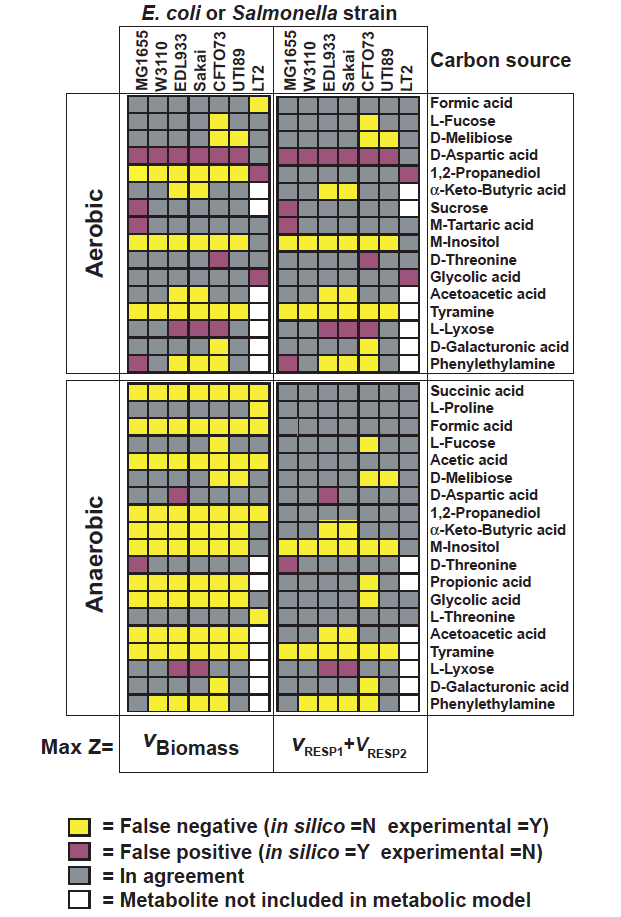
\includegraphics[width=0.4\textwidth]{images/e_coli_carbon_source} 
  \end{center}
\end{frame}